\chapter{Implementation, Integration and Test Plan}
The implementation, integration and testing of the system will follow a bottom-up approach, without omitting the dependencies between components within the same subsystem. This approach is chosen both for the server side and the client side, that will be implemented and tested in parallel. An incremental integration facilitates bug tracking and generates working software quickly during the software life cycle.\newline
External services do not need to be unit tested since it is assumed that they are reliable.

\section{Plan Definition}

\begin{figure}[H]
	\centering
	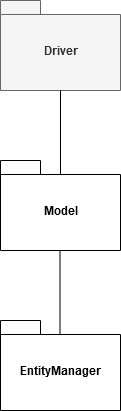
\includegraphics[width=0.15\linewidth]{bottom_up/bottom_up_1}
	\caption{Bottom-up approach first step.}
	\label{fig:bottom_up_1}
\end{figure}

\begin{figure}[H]
	\centering
	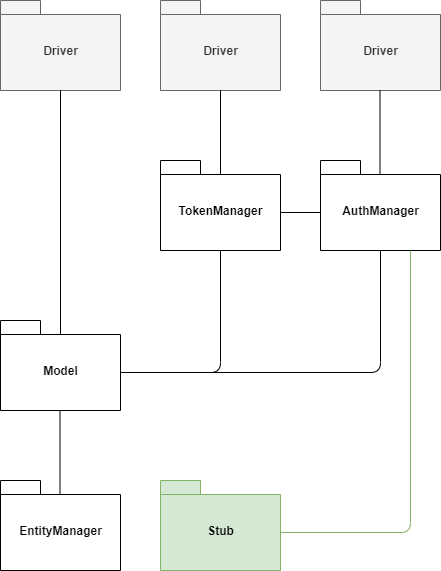
\includegraphics[width=0.5\linewidth]{bottom_up/bottom_up_2}
	\caption{Bottom-up approach second step.}
	\label{fig:bottom_up_2}
\end{figure}

\begin{figure}[H]
	\centering
	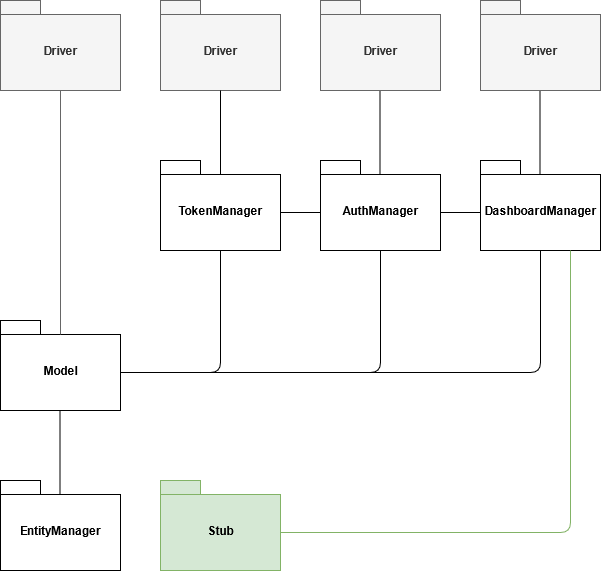
\includegraphics[width=0.75\linewidth]{bottom_up/bottom_up_3}
	\caption{Bottom-up approach third step.}
	\label{fig:bottom_up_3}
\end{figure}

\begin{figure}[H]
	\centering
	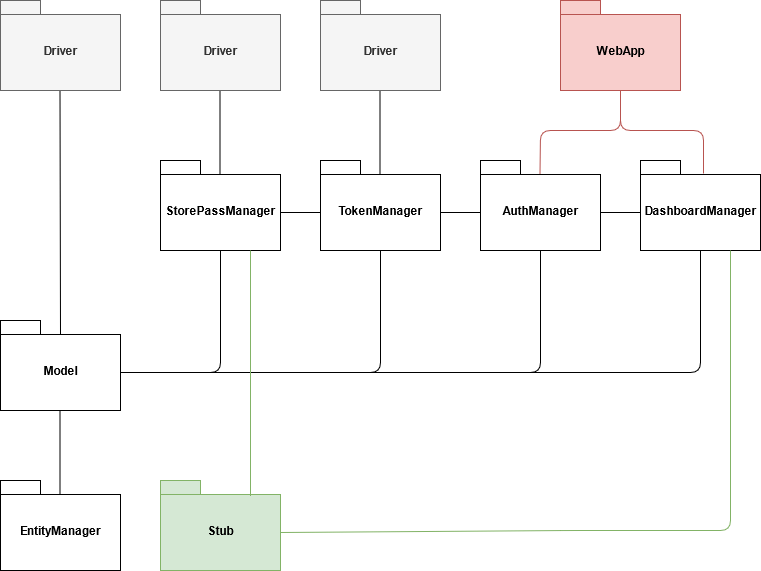
\includegraphics[width=0.75\linewidth]{bottom_up/bottom_up_4}
	\caption{Bottom-up approach fourth step.}
	\label{fig:bottom_up_4}
\end{figure}

\begin{figure}[H]
	\centering
	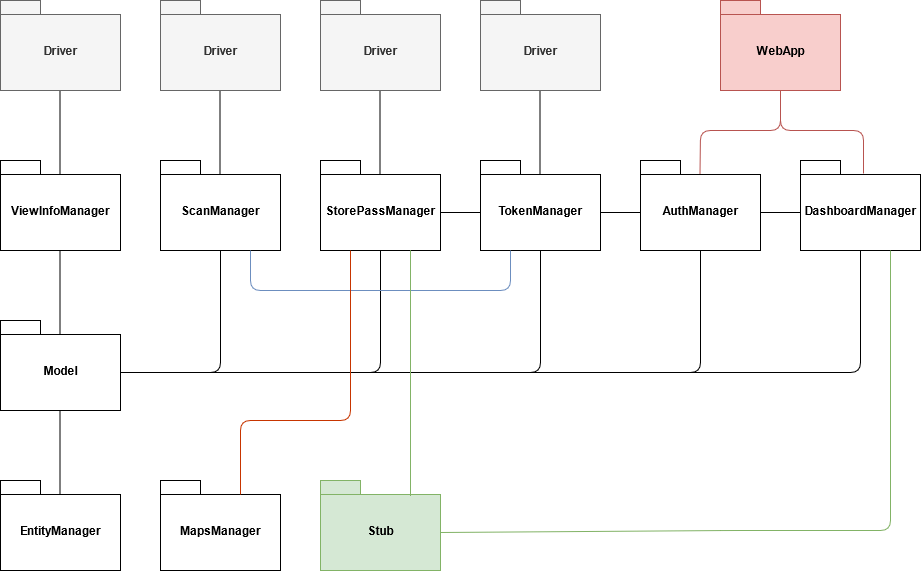
\includegraphics[width=\linewidth]{bottom_up/bottom_up_5}
	\caption{Bottom-up approach fifth step.}
	\label{fig:bottom_up_5}
\end{figure}

\begin{figure}[H]
	\centering
	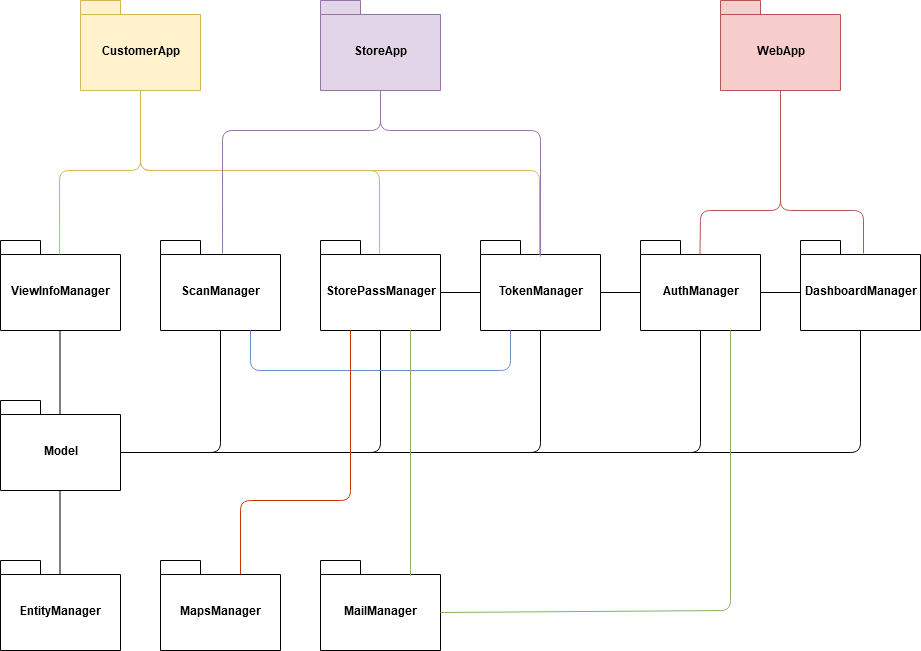
\includegraphics[width=\linewidth]{bottom_up/bottom_up_6}
	\caption{Bottom-up approach sixth step.}
	\label{fig:bottom_up_6}
\end{figure}

\clearpage

\section{Technologies}
This section will analyse the possible technologies available to develop each component of the system.

\subsection{Mobile}
The mobile applications must be accessible by as many users as possible, hence it must be developed for the major mobile OSes, Android and iOS.
In order to achieve this, it is possible to adopt a cross-platform development framework which  avoid the burden of having to use two different native codebases.
A lot of alternatives are available, most of them consisting of a web view, such as Apache Cordova and Ionic. 
However, for scalability and performance reasons, these options are discarded, in favour of a more native approach with Flutter, an open-source UI software development kit created by Google.
Since this framework compiles to native code, it provides better performance and scalability. A the same time, the availability of a big standard library of UI components avoids the need of third party packages which allows for faster development.

\subsection{Back-end server}
The back-end will be implemented in Java EE with the TomEE application/web server.
It allows for fast development and easy integration with documentation tools that help speed up the work.\newline
The web server will conform to the REST architectural design, providing a REST API, which allows for great flexibility.
 
\subsection{Front-end web app}
Java templating with Thymeleaf will be used for the web app interface.

\subsection{Database}
MySQL server is one of the world’s most popular databases. It is open source, reliable, cost-effective and easy to manage. For this reason, it is chosen for the data storage system.
